\subsubsection{\stid{6.02} LLNL ATDM Programming Models and Runtimes}


\paragraph{Overview} 
%\textit{Provide an overview of your project.  You might find that the introductory text from your Fall 2017 Project Summary \url{https://confluence.exascaleproject.org/display/1ST/Fall+2017+ECP+ST+Project+Summaries} useful as a starting draft.}
This project covers two main thrusts in programming models standards and 
runtimes for exascale supercomputing systems. The first thrust is 
programming models standards work in MPI and OpenMP. 

The Message Passing Interface Standard (MPI) is a message passing library standard based on the consensus of the MPI Forum, which has over 40 participating organizations, including vendors, researchers, software library developers, and users. The goal of the Message Passing Interface is to establish a portable, efficient, and flexible standard for message passing that will be widely used for writing message passing programs. As such, MPI is the first standardized, vendor independent, message passing library. The advantages of developing message passing software using MPI closely match the design goals of portability, efficiency, and flexibility. MPI is not an IEEE or ISO standard, but has in fact, become the ``industry standard'' for writing message passing programs on HPC platforms.

OpenMP (Open Multi-Processing) is an application programming interface (API) that supports multi-platform shared memory multiprocessing programming in C, C++, and Fortran, on most HPC platforms. To enable portable tools for performance analysis and debugging of OpenMP programs, the OpenMP Language Committee is defining application programming interfaces for tools; these interfaces are expected to be part of the OpenMP standard and supported by all OpenMP compliant implementations. There are two parts to the proposed interfaces: OMPT (a first-party API for performance tools), and OMPD (a shared-library plugin for debuggers that enables a debugger to inspect and control execution of an OpenMP program).

The other main thrust area for LLNL is the ROSE project’s work in support of 
ATDM Exascale application efforts.  
ROSE is an open source compiler infrastructure to build source-to-source program transformation and analysis tools for large-scale Fortran 77/95/2003, C, C++, OpenMP, and UPC applications. The intended users of ROSE could be either experienced compiler researchers or library and tool developers who may have minimal compiler experience. ROSE is particularly well suited for building custom tools for static analysis, program optimization, arbitrary program transformation, domain-specific optimizations, complex loop optimizations, performance analysis, and cyber-security.



\paragraph{Key  Challenges} \leavevmode \\
%\textit{Describe what is hard to do, why it is challenging.}

\textbf{ROSE.}
We will develop advanced program 
transformation and analysis to improve correctness and performance of 
RAJA codes. The research results will be communicated to RAJA maintainers to 
improve the RAJA portable programming layer. Both of these LLNL efforts 
in this area  are crucial for ECP and ASC applications to achieve portable 
performance on upcoming Exascale systems.

\textbf{MPI.}
For MPI, we focus on 
interfaces for supporting tools, including MPI\_T and MPIR, and for fault
tolerance, including Reinit. Tools for MPI are critical to ensure that
applications achieve high communication performance, and understanding
and designing fault tolerance interfaces are important for large scale
jobs on faulty systems.
The participants will follow development across the standard in
addition to the tools and fault tolerance areas. 

\textbf{OpenMP.} 
In OpenMP, our focus is on the tools interfaces 
OMPT and OMPD.  Tools are critical for application developers to understand
the correctness and performance of their codes when using OpenMP.
We will participate and monitor developments in 
all parts the standard in addition to our focus areas. 

\paragraph{Solution Strategy} \leavevmode \\
 
%\textit{Describe your basic strategy for addressing the challenges.}

\textbf{ROSE.}
The team is working to support advanced loop transformations on RAJA
code; finding loops susceptible to data races in ASC applications;
and performing performance analysis of RAJA code. ROSE improvements
will be released as open source at \url{https://github.com/rose-compiler/rose
}.

\textbf{MPI.}
LLNL staff regularly participate in regular calls and discussions for the Tools Working Group, Fault Tolerance Working Group, Sessions Working Group and attend Forum meetings that occur during the quarter.

\textbf{OpenMP.} Regularly participate in weekly OpenMP language committee calls, participate in biweekly calls of the OpenMP tools WG, email discussions on OpenMP tools interfaces (OMPD and OMPT).

\begin{figure}[htb]
        \centering
        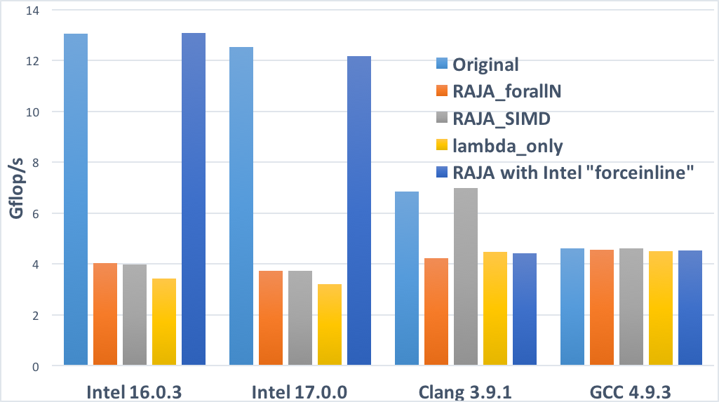
\includegraphics[width=4in]{projects/2.3.1-PMR/2.3.1.03-LLNL-ATDM-PMR/ROSE-raja}
        \caption{\label{fig:rose-raja}\textbf{Work by ROSE team shows
performance gap analysis for RAJA with different compilers.}}
\end{figure}




\paragraph{Recent Progress} \leavevmode \\

%\textit{Describe what you have done recently.  It would be good to have some kind of figure or diagram in this section.}


\textbf{ROSE.} The team continued to improve ROSE's C++11 support 
and the ROSE-based 
tool, rajaChecker. 
The team improved rajaChecker to support patterns buried deep within control 
flows. Additionally, they improved the robustness of rajaChecker and 
significantly reduced compilation errors in a large ASC application.
The team improved the tool's debugging support by adding more detailed
execution tracing information. The debugging information was used to
find the root cause of several false negative reports, which the team 
subsequently fixed. They also added new features in rajaChecker to
collect statistics about the total number of loops analyzed and how 
many loops are lambda or regular loops.



\textbf{MPI.} The MPI participants participated in the design of new 
approaches to incorporate fault tolerance in the MPI Standard, including 
standardizing primitives to support fundamental fault-tolerance methods.  
They also worked on the MPI\_T\_Events interface for tools.
The MPI participants attended the MPI Forum meetings in 2018
and proposed new approaches to incorporate fault tolerance in the 
MPI Standard, including standardizing primitives to support fundamental 
fault-tolerance methods.

\textbf{OpenMP.} In OpenMP, 
the project members attended the OpenMP 
face-to-face meeting in Austin and worked with the Tools subcommittee 
to prepare and enact several tickets to improve OMPT and OMPD 
specifications. In particular, they improved the OMPD prototype for
NVIDIA GPUs and the clang/LLVM runtime. They also updated the OMPD
prototype runtime to be fully compliant with OpenMP 5.0.


\paragraph{Next Steps}  \leavevmode \\


\textbf{ROSE.} Continue to improve ROSE support for RAJA and ASC applications.

\textbf{MPI.} Continue to participate in MPI Forum on fault tolerance and
tools.

\textbf{OpenMP.} Continue to participate in OpenMP Standards Committee
on tools and debuggers.
